	\section{Methods}

\subsection{Existing methods}

\subsection{Proposed methods}

\subsection{RSSI proximity detection}

\begin{figure}[!t]
	\centering
	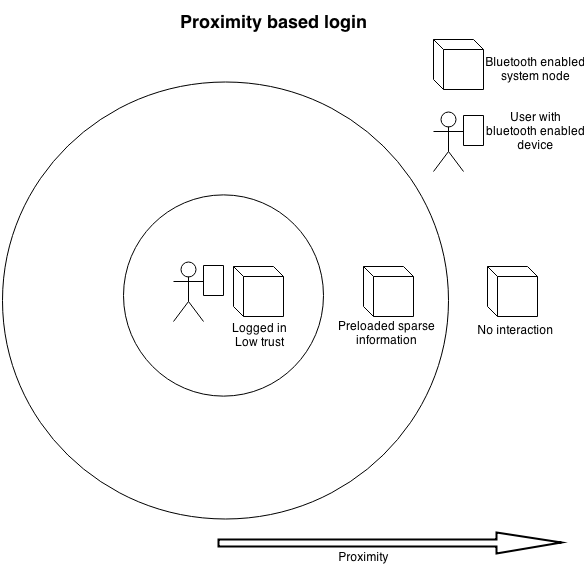
\includegraphics[width=2.5in]{img/proximityBasedLogin}
	\caption{ Proximity based login }
	\label{fig_proximity_based_login}
\end{figure}

When the strength of a RSSI signal reaches a predefined high threshold, when measured from the system, the user is sufficiently close to interact with the system, and the user will be partially authenticated.
When a user has been authenticated but decides to move away from the system the user will be deauthenticated when the RSSI reaches a predefined low threshold.

Furthermore it is possible to preload information about earlier sessions when a user is moving towards the system.
When the user is close enough to be partially authenticated the system thus has preloaded information and may be able to present additional relevant data based on the preloaded information from earlier sessions. 
\cref{fig_proximity_based_login} illustrates the concept of preloading information based on the users proximity to the system.

\subsection{Bluetooth Low Energy authentication}

\subsection{Partial authentication model}
A login method has been developed to take different levels of trust into account.
As presented in \cref{fig_authentication_model} the authentication model has three levels of trust
\begin{itemize}
\item High (green)
\item Medium (yellow)
\item Low (red)
\end{itemize}

\begin{figure}[!t]
	\centering
	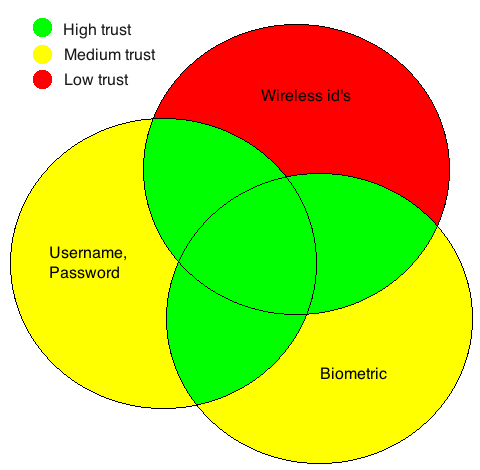
\includegraphics[width=2.5in]{img/authenticationModel}
	\caption{ Partial login and trust }
	\label{fig_authentication_model}
\end{figure}

High trust is obtained by authenticating with a combination of two of the three authentication methods.
As shown in \cref{table_data_access} a user is only able to view and edit sensitive data within the high trust area of the model.

Medium trust is obtained by authenticating with either a username/password or biometric authentication.
These two authentication methods is reasonable secure and are used universally for authentication.
A user that has obtained medium trust is able to view sensitive data but cannot edit or delete it.
With medium trust a user can view and edit non sensitive data.

Low trust is obtained by calm authentication with a Bluetooth enabled device.
A user with low trust can view personal non sensitive data like a name or a personal todo-list.
No edit or delete is allowed.

This model allows the user to be partially authenticated before any physical interaction.
The system gets the ability to recognize users and may for instance use that information to move a session started on one system to the current system so the user is able to seamlessly work on from the point the previous session ended.

\begin{table}[!t]
\caption{Data access}
\label{table_data_access}
\centering
% Some packages, such as MDW tools, offer better commands for making tables
% than the plain LaTeX2e tabular which is used here.
\begin{tabular}{|p{1.3cm}|p{2.0cm}|p{2.0cm}|p{2.0cm}|}
\hline
\textbf{Trust} & \textbf{Non sensitive personal data} & \textbf{Non sensitive data} & \textbf{Sensitive data}\\
\hline
\textbf{High} & Read/Write & Read/Write & Read/Write\\
\hline
\textbf{Medium} & Read/Write & Read/Write & Read\\
\hline
\textbf{Low} & Read & - & -\\
\hline
\end{tabular}
\end{table}